\documentclass[eng,printmode]{mgr}
\usepackage{polski}
\usepackage{url}
\usepackage{listings}
\usepackage[utf8]{inputenc}
\usepackage[T1]{fontenc}
\usepackage{scrextend}
\usepackage{graphicx}
\usepackage{subfigure}
\usepackage{psfrag}
\usepackage{float}
\usepackage{amsmath}
\usepackage{amsfonts}
\usepackage{enumitem}
\usepackage{supertabular}
\usepackage{array}
\usepackage{tabularx}
\usepackage{hhline}
\usepackage{graphicx}
\graphicspath{ {./img/} }
\usepackage{showlabels}
\usepackage{tabu}
\newcommand{\R}{I\!\!R}
\newtheorem{theorem}{Twierdzenie}[section]

\title{Porównanie metod wykrywania obserwacji odstających w danych teleinformatycznych}
\engtitle{Comparsion of outliers detecting methods in ICT data}
\author{Maciej Bakowicz}
\supervisor{prof. dr hab. inż. Krzysztof Walkowiak, W-4}

\field{Teleinformatyka (TIN)}
\specialisation{Projektowanie Sieci Teleinformatycznych (TIP)}


\begin{document}
\bibliographystyle{plain}
\maketitle 

\tableofcontents 

\chapter{Wstęp}  
Obserwację odstającą można zdefiniować jako punkt lub zbiór punktów, które swoimi wartościami różnią się od wartości punktów je otaczających. Obserwację taką można definiować lokalnie, gdzie anomalie to pojedyncze punkty a zbiorem porównawczym są punkty w bliskim sąsiedztwie lub bardziej globalnie, gdzie do analizy konkretnych przedziałów potrzebna jest wiedza o całym zbiorze (np. analiza miesięcznego trendu w danych ze stemplem czasowym). 
\\ \\
Występowanie danych odstających (anomalii, outliers) jest jednym z najczęściej spotykanym problemem w środowisku zajmującym się zbieraniem oraz analizą danych. Każde przeprowadzone badanie posiada odchyły w danych, miejsca, które nie pasują do ogólnie ukształtowanego trendu. Widać to szczególnie w środowiskach mniej kontrolowanych, takich, w których występowanie czynników zewnętrznych jest duże i nieprzewidywalne (duży rozrzut losowości). \\ \\
Występowanie tego typu anomalii ma negatywny wpływ na proces analizy i przygotowania takiego zbioru danych. Powoduje to bowiem, że rozkład zbioru danych jest przekłamany - z powodu występowania zawyżeń lub zaniżeń takich miar jak średnia czy mediana. Z punkty widzenia statystyki nieciągły, niejednorodny czy też niespójny zbiór danych nie może być wiarygodny i rzetelny \cite{outliers-impact}.
\\ \\
Kolejnym powiązanym problem jest problem zarządzania wykrytymi już anomaliami. Zazwyczaj stosuje się dwie metody: próba naprawienia punktu lub jego usunięcie. W zależności od charakteru i genezy danych można wykonać obie operacje, jedną z nich lub żadną. Podjęcie takiej decyzji wiąże się bezpośrednio z tym co jest badane oraz do czego tego typu zbiór danych będzie wykorzystywany. \\
Naprawa zazwyczaj polega na wykorzystaniu statycznych miar takich jak wartość średnia, mediana czy odchylenie standardowe. Istnieje wiele sprawdzonych i opublikowanych metod do tego służących. \\
Zazwyczaj do naprawy i usunięcia potrzebna jest konkretna wiedza o prawdopodobnych i dozwolonych wartościach w zbiorze. Innymi słowy, sama algorytmiczna klasyfikacja punktu jako odstającego nie jest wystarczająca, żeby podjąć jakiekolwiek kroki mające na celu ingerencję w zbiór danych. 
\\ \\ 
Ze względu na specyfikę danych w pracy nie zostanie podjęta jakakolwiek próba ingerencji w zbiór danych w celu naprawy / usunięcia.

\section{Cel pracy}
Celem niniejszej pracy jest zaprojektowanie oraz zaimplementowanie systemu, który w efektywny sposób wykryje błędy (tu: znaczące odstępstwa od normy w przedziale lokalnym) w danych tyczących się infrastruktury teleinformatycznej (głównie stacje nadawczo-odbiorcze BTS - Base Transceiver Station). W czasie realizacji pracy zostaną zaimplementowane istniejące oraz własne algorytmy a następnie porównane między sobą w celu wybrania sposobu (algorytmu) optymalnego. Zaprojektowany system nie powinien sam ingerować w dane (usuwać, zmieniać), gdyż dane nie są obarczone informacjami dodatkowymi (jak chociażby przerwy w działaniu stacji bazowych) przez co nie ma wystarczającej wiedzy potrzebnej do stwierdzenia przyczyny wystąpienia błędu. W końcowej fazie projektu system powinien móc wskazać błędne dane a następnie przedstawić użytkownikowi możliwości, gdzie w zależności od natury, charakteru użytkownik mógłby je usunąć lub spróbować naprawić (ręcznie lub za pomocą algorytmów uczenia maszynowego). 

\section{Zakres pracy}
\subsection{Przygotowanie danych}
Pierwszym etapem niniejszej pracy jest zebranie rzeczywistych danych od firmy zajmującej się ich zbieraniem i przetwarzaniem.  \\
Wartości oraz opisy pewnych cech tych danych są w dużej mierze tajne i zawierają poufne informacje, dlatego przedstawienie ich w niezmienionej formie byłoby poważnym naruszeniem umowy oraz klauzuli poufności zawartych z firmą. \\
Dlatego kolejnym krokiem jest zaprogramowanie algorytmu, programu, który będzie w stanie zmienić strukturę tych danych, w szczególności przypisać nazwy rzeczywistych operatorów oraz identyfikatorów urządzeń zbierających dane do nazw losowych, którymi posługiwać będzie można się w sposób swobodny w dalszych etapach pracy. \\
Zdobyte dane zawierają również szereg dodatkowych informacji, które powinny zostać odrzucone ze względu na małą wartość informacyjną i zachowanie ich jest niepotrzebne do realizacji celu pracy. Dlatego kolejnym i ostatnim krokiem w przygotowaniu danych jest stworzenie nowych struktur, tabel i schematów a następnie przekopiowanie tych wartości, które są niezbędne. Ilość danych (około pół miliona wierszy) jest na tyle duża, że wykorzystanie mechanizmów do zarządzania Big Data jest niezbędne \cite{cassandra}\cite {cassandra-driver}.

\subsection{Wybór technologii i algorytmów}
Po utworzeniu struktur i wypełnieniu ich danymi kolejnym krokiem jest wybranie istniejących już algorytmów wykrywania obserwacji odstających \cite{outliers-basic} a następnie ich implementacja w wybranym języku programistycznym lub wykorzystanie rozwiązań już wcześniej zaimplementowanych. Ilość zaimplementowanych algorytmów zależy w dużej mierze od stopnia trudności w ich implementacji oraz testowaniu a także od ilości dostępnych materiałów na ich temat. W obrębie wyboru algorytmów znajdzie się zatem nie tylko ich wyszukanie i implementacja ale także wstępna segregacja wraz z odrzuceniem tych mniej obiecujących czy nie pasujących do koncepcji. Część zaimplementowanych algorytmów może w końcowym etapie nie być brane pod uwagę ze względu właśnie na ich mniejszą użyteczność. \\
Najbardziej obiecującą technologią jest język Python \cite{python} ze względu na dużą ilość bibliotek do tworzenia struktur i schematów danych \cite{pandas} a także działań matematycznych co uproszcza proces pisania algorytmów \cite{numpy}.

\subsection{Napisanie własnego algorytmu}
Po zaimplementowaniu i przetestowaniu istniejących już rozwiązań oraz analizie ich wyników zostanie zaimplementowany własny algorytm, który wykorzystuje autorskie rozwiązania. Aby w procesie porównywania algorytmów wyniki były rzetelne i porównywalne rozwiązania te muszą wykorzystywać podobne mechaniki co wcześniej wybrane algorytmy \cite{isolation-forest}\cite{novelty}. 

\subsection{Stworzenie raportu porównawczego}
Końcowym etapem pracy jest napisanie raportu porównawczego oraz wybór cech, które będą ze sobą porównywane. Raport ten zawiera szereg porównań między kolejnymi algorytmami wraz ze wskazaniem tego optymalnego w zależności od przypadku użycia. Algorytmy są testowane kilkukrotnie na różnych zestawach danych (różniącymi się charakterystykami oraz wartościami). \\
Na potrzeby lepszej wizualizacji porównań oraz działania poszczególnych algorytmów do raportu zostaną dołączone spore ilość wykresów, data gramów oraz tabel \cite{react}\cite{react-chart}.

\chapter{Przegląd literatury}
Specyfika dostarczonych danych, które są wykorzystywane do przeprowadzenia badań i symulacji wybranych metod narzuca pewne ograniczenia co do wyboru i wykorzystania algorytmów. Z powodu braku jakichkolwiek wzorcowych zbiorów danych, które mogłyby posłużyć jako zbiory uczące. \\
Wybrane algorytmy zatem powinny mieć możliwość klasyfikacji zbioru danych (podziału wg. określonych cech) a następnie na podstawie określonego warunku i parametrów określały punkty odstające.

\section{Metoda okna czasowego}
Metoda okna czasowego jest to sposób podziału całego zbioru danych na szereg mniejszych zbiorów zawierających się w pojedynczym, z góry określonym wycinku czasowym (dziedzina funkcji).\\
Podział określają dwa parametry:
\begin{itemize}
\item szerokość okna - ilość punktów dla podzbiorów wygenerowanych z podanego zbioru danych
\item długość kroku - ilość punktów o które okno jest przesuwane w każdej iteracji
\end{itemize}

Startowa pozycja okna to punkt 0 na osi X (dziedzina). Okno przesuwa się w prawą stronę. Dopuszczalne jest aby ostatni podzbiór miał inną szerokość niż przyjęta na początku (wynika to z niekoniecznie całkowicie podzielnego zbioru danych na równe podzbiory).
\\ \\
Działanie metody wizualizuje poniższy rysunek.
\\
\begin{figure}[h]
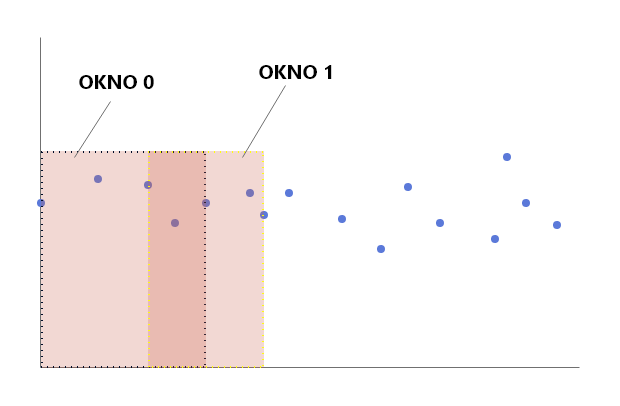
\includegraphics[scale=0.6]{okno_czasowe}
\caption{Działanie metody podziału na okna czasowe}
\end{figure}
\\
Szerokość okna przyjęto jako 5 a długość kroku jako 2. Można zauważyć, że okna różnią się obszarem zajmowanej dziedziny co wynika z niejednorodnego rozrzutu punktów.
\\
Dodatkowo widać, że istnieją części wspólne dla sąsiadujących podzbiorów. Zastosowanie okna czasowego w tej postaci, zapewni, że większość punktów może być analizowana w różnych środowiskach, przez co eliminuje się lokalne odchylenia, istniejące jedynie w jednym z podzbiorów.
\\
W zależności od zastosowanego algorytmu na podzbiorach metoda ta powinna dzielić zbiór danych na co najmniej 10 podzbiorów lecz należy pamiętać, że ilość punktów w danym podzbiorze (szerokość okna) nie powinna być mniejsza niż 2-5 procent szerokości całego zbioru danych.
\\
Zastosowanie tej metody zatem jest opłacalne jedynie, gdy badany zbiór danych posiada sporą ilość wartości (liczonych w setkach). Dla mniejszych zbiorów danych stosowanie tej metody nie ma sensu. 
\section{Algorytm K-Mean}
Algorytm opierający swoje działanie na podziale zbioru danych na podzbiory nazywane klastrami (ang. clusters). Przydział punktów do konkretnego klastra polega na obliczaniu jego odległości względem punktów sąsiednich (odległość euklidesowa). \\ \\
Algorytm przyjmuje wiele parametrów, jednak najważniejszym jest ilość klastrów, na które należy podzielić zbiór danych.

Podział na klastry definiuje również pojęcie centroidów (ang. centroids), które przyjmują wartości środka wyznaczonych klastrów (każdy klaster posiada jeden centroid). \\ \\

Podział serii danych ze stemplem czasowym na pojedyncze klastry wraz z centroidami można zobaczyć na poniższym rysunku:
\\
\begin{figure}[h]
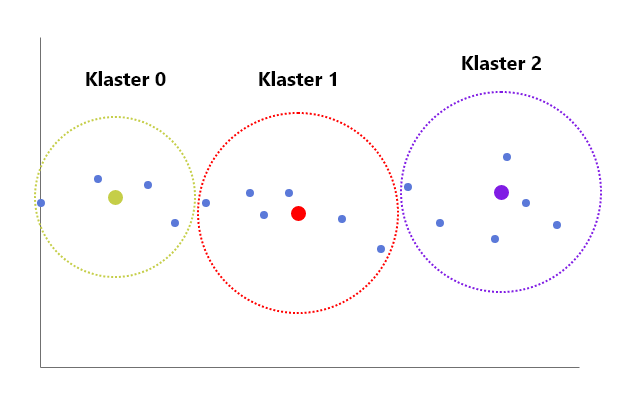
\includegraphics[scale=0.6]{KMean}
\caption{Klasyfikacja zbioru danych}
\end{figure}
\\
Informację o przynależności punktu do konkretnego klastra można wykorzystać do wyznaczenia punktów odstających lokalnie (w jednym klastrze). \\
Sam stempel czasowy jest cechą słabą (jest ona różna dla każdego punktu), dlatego przy stosowaniu tej metody należy rozważyć przypisanie cech dodatkowych, dzięki którymi podział na klastry będzie bardziej dokładniejszy.
\subsection{Wykorzystanie całych klastrów}
\subsection{Wykorzystanie odległości od centroidu}
\section{Algorytm regresji liniowej}
\section{Algorytm Isolation Forest}

\chapter{Opis architektury}
\section{Specyfikacja danych wejściowych}
Zbiór danych, który zostanie wykorzystany do zrealizowania zadania odnajdywania obserwacji odstających jest przedstawiony w uporządkowanej strukturze, która na potrzeby pracy została przeorganizowana (niektóre pola zostały usunięte ze względu na ich nieużyteczność) oraz przeredagowana (wartości niektórych pól zostały podmienione - na podstawie wcześniej stworzonego słownika - w celu ukrycia informacji wrażliwych). Dodatkowo powstało kilka struktur pomocniczych.
\\

\subsection{raw\_data}
Zbiór wszystkich punktów wartości, które zostały zmierzone. Jest to podstawowa struktura, z której danej posłużą wyszukiwaniu obserwacji odstających. Struktura ta zawiera wszystkie, nieprzypisane dane. Proces przypisywania i wyodrębniania danych, które dotyczą tego samego źródła zachodzi na bieżąco w czasie działania algorytmu. Tworzenie osobnych struktur (tabel w bazie danych) dla każdego źródła osobno byłoby mało optymalne i nieelastyczne (np. w sytuacji gdy dochodzą nowe "paczki" danych).
\\

\begingroup
\fontsize{10pt}{12pt}\selectfont

\begin{tabu} to 0.9\textwidth { | X[l] | X[l] | X[l] | X[l] | X[l] |}
\hline
\textbf{operator\_id} & \textbf{acronym} & \textbf{kpi\_name} & \textbf{date} & \textbf{value}\\
\hline
\textit{Long}  & \textit{Text}  & \textit{Text} & \textit{Timestamp} & \textit{Long} \\
\hline
364 & CANADA\_818 & KPI\_1 & 2015-10-30 10:45 UTC & 93.31 \\
\hline
\end{tabu}
\endgroup
\\
\\

\noindent \textbf{operator\_id} - numer identyfikujący operatora, którego dane dotyczą
\\\\
\textbf{acronym} - logiczny identyfikator wskazujący na pochodzenie danych (określający fizyczną lokalizację źródła danych)
\\\\
\textbf{kpi\_name} - nazwa określająca rodzaj urządzenia, które pomiar wykonało. Urządzenie to posiada dodatkowe cechy takie jak jednostka, co jest mierzone (jaki typ danych), jednak nie zostało to w tej strukturze uwzględnione, gdyż proces przetwarzania danych wymaga bardziej skomplikowanych definicji. Zostało to uwzględnione w dalszych strukturach danych.
\\\\
\textbf{date} - punkt w czasie, w którym pomiar został przeprowadzony. Może być to dokładna data lub data wskazująca na zakres dat (np. jeden dzień)
\\\\
\textbf{value} - wartość liczbowa dla tego punktu w danym czasie (tak samo jak dla daty, może to być wartość dla konkretnego punktu w czasie lub uśredniona wartość zebranych wartości z konkretnego okresu czasu).
\\ \\
Przykładową strukturę oraz źródła pochodzenia reprezentuje poniższy rysunek.
\begin{figure}[h]
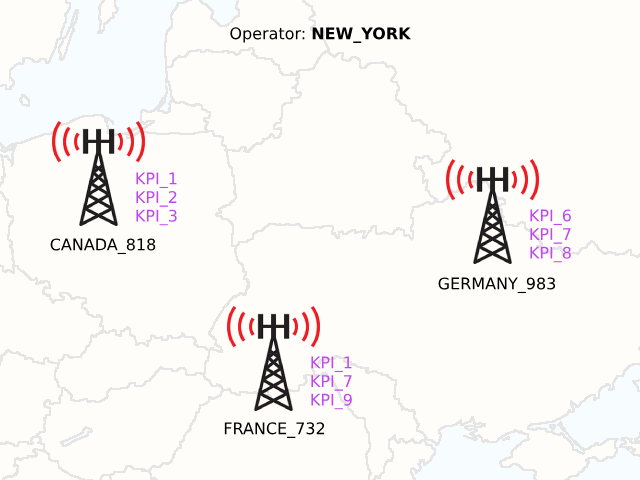
\includegraphics[scale=0.6]{struct}
\caption{Przykładowa struktura podziału sieci}
\end{figure}
\\
Powyższa struktura w bazie danych wyglądałaby następująco:
\\\\
\begingroup
\fontsize{10pt}{12pt}\selectfont
\begin{tabu} to 0.9\textwidth { | X[l] | X[l] | X[l] | X[l] | X[l] |}
\hline
\textbf{operator\_id} & \textbf{acronym} & \textbf{kpi\_name} & \textbf{date} & \textbf{value}\\
\hline
364 & CANADA\_818 & KPI\_1 & 2015-10-30 00:00 UTC & 120.72 \\
\hline
364 & CANADA\_818 & KPI\_2 & 2015-10-31 00:00 UTC & 90.81 \\
\hline
364 & CANADA\_818 & KPI\_3 & 2015-11-01 00:00 UTC & 1483 \\
\hline
364 & FRANCE\_732 & KPI\_1 & 2015-10-30 00:00 UTC & 112.21 \\
\hline
364 & FRANCE\_732 & KPI\_7 & 2015-10-31 00:00 UTC & 121.2 \\
\hline
364 & FRANCE\_732 & KPI\_9 & 2015-11-07 00:00 UTC & 910.01\\
\hline
364 & GERMANY\_983 & KPI\_6 & 2015-10-31 00:00 UTC & 0 \\
\hline
364 & GERMANY\_983 & KPI\_7 & 2015-11-10 00:00 UTC & -1 \\
\hline
364 & GERMANY\_983 & KPI\_8 & 2015-12-29 00:00 UTC & 0.11 \\
\hline
\end{tabu}
\endgroup
\\

\subsection{kpi\_definitions}
Zbiór pomocniczy opisujący podstawowe cechy KPI. Zbiór ten nie wpływa na wyniki badań, może być jednak pomocny w procesie decyzyjnym (decyzja o uznaniu punktów odstających jako błędnych oraz usunięciu lub poprawieniu ich). W sytuacji gdy zbiór punktów określany przez definicję jest wyrażony w procentach decyzję o usunięciu / poprawieniu punktów można oprzeć na prostym założeniu, że punkty poza zakresem 0 - 100 są uznawane jako błędne.
\\

\begingroup
\fontsize{10pt}{12pt}\selectfont

\begin{tabu} to 0.9\textwidth { | X[l] | X[l] | X[l] | }
 \hline
 \textbf{formula} & \textbf{title} & \textbf{description}\\
 \hline
 \textit{Text}  & \textit{Text}  & \textit{Text} \\
\hline
 [KPI\_1/ 1000]  & Call interrupt measure  & Number of interrupted calls during the day \\
\hline

\end{tabu}
\endgroup
\\\\

\noindent\textbf{formula} - matematyczna formuła (równanie) złożona z jednego lub wielu \textit{kpi\_name}. Określa jak należy liczyć i interpretować wartości końcowe (np. jeden operator obserwuje zachowanie się sieci w różnych punktach geograficznych a następnie interpretuje średnią wartość jako wartość poprawną dla obszaru, który znajduje się w zasięgu sieci). Na potrzeby pracy formula składa się \textbf{z tylko jednego} kpi\_name, toteż dodatkowe przeliczenia nie są potrzebne co stanowczo uproszcza proces agregacji i wyszukiwania.
\\\\
\textbf{title} - tytuł definicji, używany jedynie dla lepszej reprezentacji danych po stronie użytkownika.
\\\\
\textbf{description} - krótki opis definicji, określający jakiego typu danych dotyczy przeprowadzony pomiar.

\subsection{operators}
Zbiór danych w postaci prostego słownika określającego nazwę operatora oraz jego unikalny identyfikator. Użyty w procesie początkowej anonymizacji danych.
\\

\begingroup
\fontsize{10pt}{12pt}\selectfont

\begin{tabu} to 0.9\textwidth { | X[l] | X[l] | }
 \hline
 \textbf{operator\_id} & \textbf{operator\_name}\\
 \hline
 \textit{Long}  & \textit{Text} \\
\hline
 364  & NEW\_YORK \\
\hline
\end{tabu}
\endgroup
\\\\

\noindent\textbf{operator\_id} - unikalny identyfikator operatora
\\\\
\textbf{operator\_name} - przyjazna użytkownikowi nazwa operatora. Podmieniona na nazwę losowego miasta w procesie anonymizacji.


\subsection{operator\_to\_acronym\_kpi}
Zbiór danych określający wszystkie występujące kombinacje trójki \textit{operator, acronym, kpi\_name}. Stworzenie tej struktury wynikało ze specyfiki użytej bazy danych (Cassandra DB), która wymaga podania wszystkich trzech kluczy do otrzymania pozostałych wartości wiersza.
\\
\begingroup
\fontsize{10pt}{12pt}\selectfont

\begin{tabu} to 0.9\textwidth { | X[l] | X[l] | X[l] | }
 \hline
 \textbf{operator\_id} & \textbf{acronym} &\textbf{kpi\_name}\\
 \hline
 \textit{Long}  & \textit{Text}  & \textit{Text} \\
\hline
 364  & CANADA\_818 & KPI\_1\\
\hline
\end{tabu}
\endgroup
\\\\

\subsection{operator\_aliases}
Słownik opisujący translację rzeczywistych nazw operatorów na nazwy przypisanych aliasów (nazw miast). Struktura ta jest potrzebna do odtworzenia i uzupełnienia struktury w procesie anonymizacji (np. w momencie uruchamiania środowiska na nowo lub w momencie otrzymania nowych zbiorów danych).
\\
\begingroup
\fontsize{10pt}{12pt}\selectfont

\begin{tabu} to 0.9\textwidth { | X[l] | X[l] | }
 \hline
 \textbf{raw} & \textbf{alias}\\
 \hline
 \textit{Text}  & \textit{Text} \\
\hline
 T-Mobile  & NEW\_YORK \\
\hline
\end{tabu}
\endgroup
\\\\

\subsection{acronym\_aliases}
Analogiczna struktura do \textit{operator\_aliases} jednak tycząca się rzeczywistych wartości dla \textit{acronym}. Za aliasy posłużyły nazwy krajów.
\\
\begingroup
\fontsize{10pt}{12pt}\selectfont

\begin{tabu} to 0.9\textwidth { | X[l] | X[l] | }
 \hline
 \textbf{raw} & \textbf{alias}\\
 \hline
 \textit{Text}  & \textit{Text} \\
\hline
 LTE\_818  & CANADA\_818 \\
\hline
\end{tabu}
\endgroup
\\\\

\section{Pochodzenie danych wejściowych}
Powyższe zbiory / struktury danych są rezultatem zbierania i agregowania danych z wielu źródeł jednocześnie. Dodatkowo dane otrzymane od firmy zostały wcześniej maszynowo uporządkowane (poprzez wykorzystanie licznych narzędzi i algorytmów). Wykorzystane dane w pracy nie są zatem otrzymane bezpośrednio. Tak duża różnorodność oraz ilość podejmowanych w stosunku do tych danych działań skutkuje licznymi błędami w nich (błędy, których wykrycie jest zadaniem niniejszej pracy). Z pośród wielu przyczyn tych błędów można wskazać kilka najczęściej występujących:
\begin{itemize}
\item \textbf{Błąd ludzki} - duży procent "paczek" danych jest przetwarzanych, sortowanych, dopasowywanych do odpowiednich baz danych przez ludzi. Dodatkowo często dochodzi do nieporozumień na etapie uzgadniana wartości i procesów biznesowych. Rezultatem tego są - zazwyczaj - długie przedziały niepasujących danych (trudniejsze do wykrycia maszynowo bez dodatkowych informacji ze względu na utrzymujący się trend).
\item \textbf{Błąd w algorytmach} - otrzymane dane zostały wzięte z jednej z wielu baz wykorzystywanych w firmie. Dane te często są częściowo lub w całości skopiowane z bazy innego systemu, który wykorzystuje wiele algorytmów dopasowywania danych w odpowiednie miejsca. Istnieją przypadki gdzie bazując na słownikach występuje decyzja o przypisaniu danych np. do odpowiedniego operatora, bardzo często zawierając instrukcje warunkowe, które nieaktualizowane z czasem powodują złe przypisania (zazwyczaj pojedyncze punkty).
\item \textbf{Uszkodzenia mechaniczne urządzeń} - możliwym przypadkiem są również wszelkiego rodzaju uszkodzenia sieci. Raportowane wówczas dane zawierają wszelkiego rodzaju przekłamania, różnice okresowe (zazwyczaj krótkie okresy).
\end{itemize}
\section{Specyfikacja danych wyjściowych}
Przetworzone przez algorytmy zbiory danych zostaną poetykietowane i posegregowane na dwa zbiory punktów:
\begin{itemize}
\item Punkt odstający - potencjalny punkt odstający swoją wartością od pozostałych z tego samego zbioru
\item Punkt poprawny - punkt sklasyfikowany jako należący do zbioru (punkt nieodstający)
\end{itemize}

Reprezentacja w bazie danych wygląda następująco:
\\
\begingroup
\fontsize{10pt}{12pt}\selectfont

\begin{tabu} to 0.9\textwidth { | X[l] | X[l] | X[l] | X[l] | X[l] | X[l] |}
\hline
\textbf{operator\_id} & \textbf{acronym} & \textbf{kpi\_name} & \textbf{date} & \textbf{value} & \textbf{is\_outlier}\\
\hline
\textit{Long}  & \textit{Text}  & \textit{Text} & \textit{Timestamp} & \textit{Long} & \textit{Boolean}\\
\hline
364 & CANADA\_818 & KPI\_1 & 2015-10-30 10:45 UTC & 93.31 & True\\
\hline
\end{tabu}
\endgroup

\section{Przeznaczenie danych wyjściowych}
Z powodu braku konkretnych informacji dodatkowych opisujących zachowanie się sieci czy specyfiki zbiorów danych wykryte obserwacje odstające można jedynie przekazać do dalszej analizy.\\
Rezultaty oczywiście mogą zostać przeprocesowane metodami do usuwania i korekcji danych jednak w tym przypadku nie ma żadnej pewności, że rezultat będzie poprawny czy w ogóle pożądany, bowiem charakterystyka danych jest na tyle specyficzna, że bez równie specyficznej wiedzy nie ma stu procentowej pewności na zgodność z oczekiwaniami.

\bibliography{bibliografia}
\end{document}